\begin{figure}
	\centering
	\subfigure[$\Delta t$ = 1 día]{
	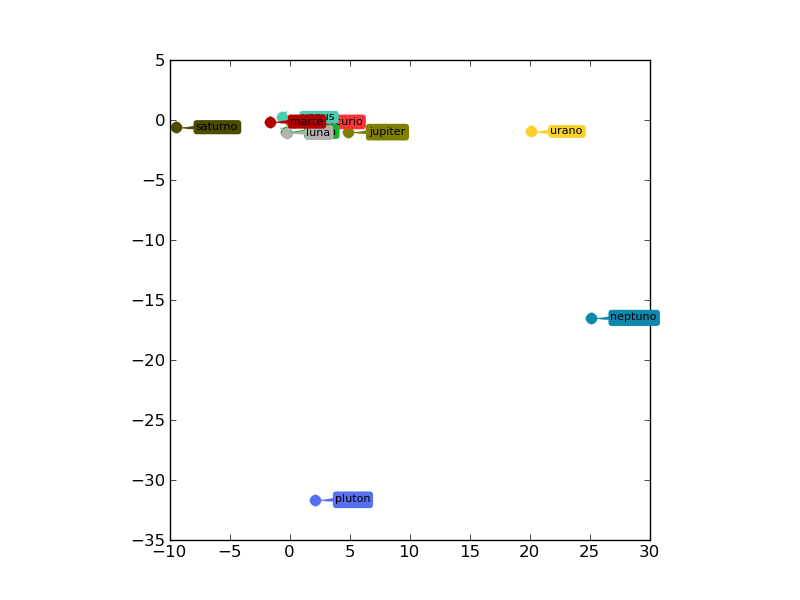
\includegraphics[scale=0.38]{img/ej2/metodo_2/validacion_30_1.png}
	\label{fig:ej2_m2_30_1}
	}
	\subfigure[$\Delta t$ = 6 horas]{
	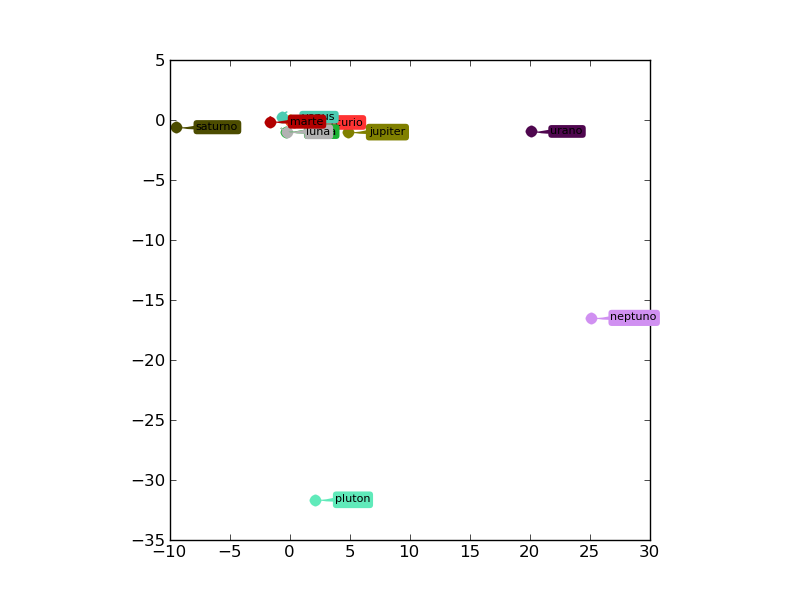
\includegraphics[scale=0.38]{img/ej2/metodo_2/validacion_30_4.png}
	\label{fig:ej2_m2_30_4}
	}
	\\
	\subfigure[$\Delta t$ = 2 horas]{
	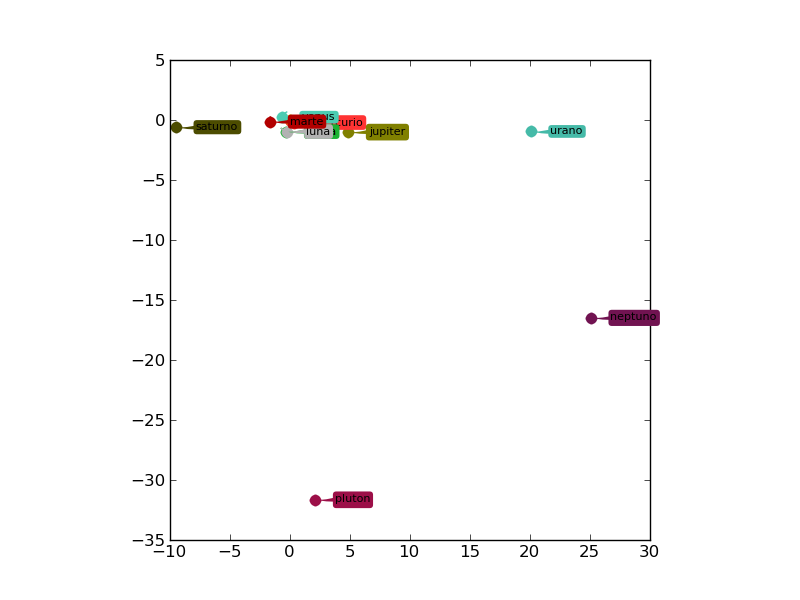
\includegraphics[scale=0.38]{img/ej2/metodo_2/validacion_30_12.png}
	\label{fig:ej2_m2_30_12}
	}
	\subfigure[$\Delta t$ = 1 hora]{
	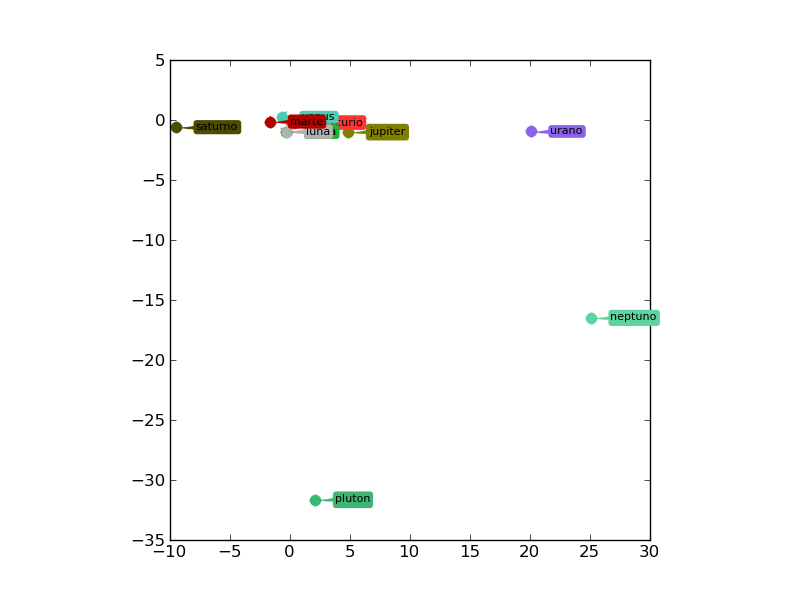
\includegraphics[scale=0.38]{img/ej2/metodo_2/validacion_30_24.png}
	\label{fig:ej2_m2_30_24}
	}
	\caption{
		Simulación de validación del sistema solar para un período de 30 días y distintos $\Delta t$
		con el método 2.
		Observamos que el error no parece ser tan grande a simple vista para este período.
	}
	\label{ fig:res_ej2_m2_30 }
\end{figure}
\begin{figure}
	\centering
	\subfigure[$\Delta t$ = 1 día]{
	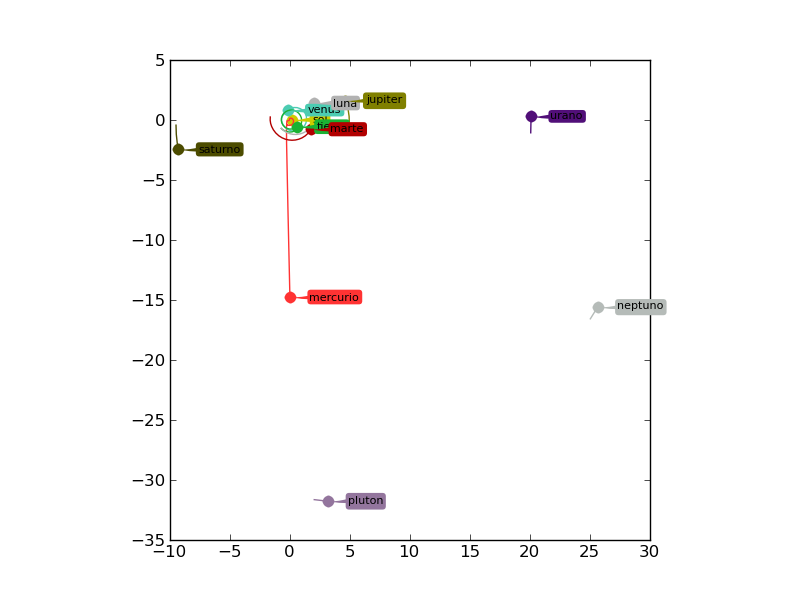
\includegraphics[scale=0.38]{img/ej2/metodo_2/validacion_365_1.png}
	\label{fig:ej2_m2_365_1}
	}
	\subfigure[$\Delta t$ = 6 horas]{
	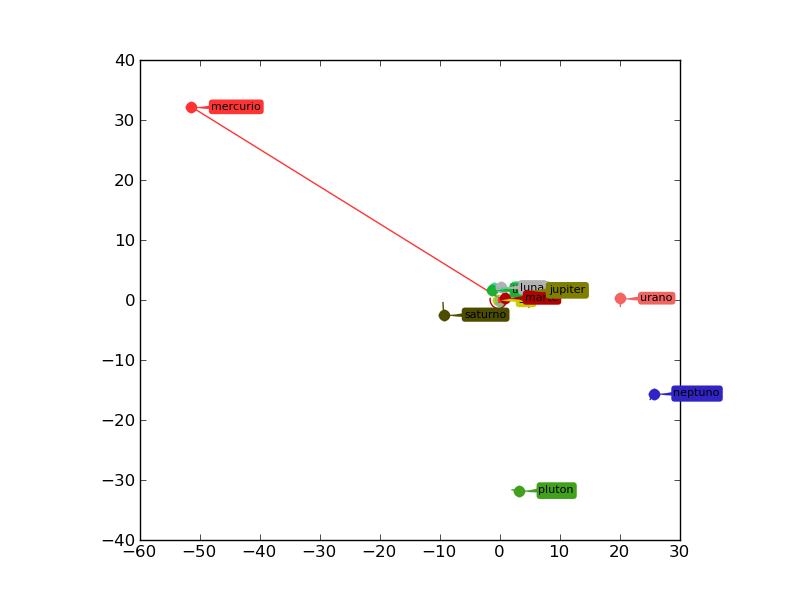
\includegraphics[scale=0.38]{img/ej2/metodo_2/validacion_365_4.png}
	\label{fig:ej2_m2_365_4}
	}
	\\
	\subfigure[$\Delta t$ = 2 horas]{
	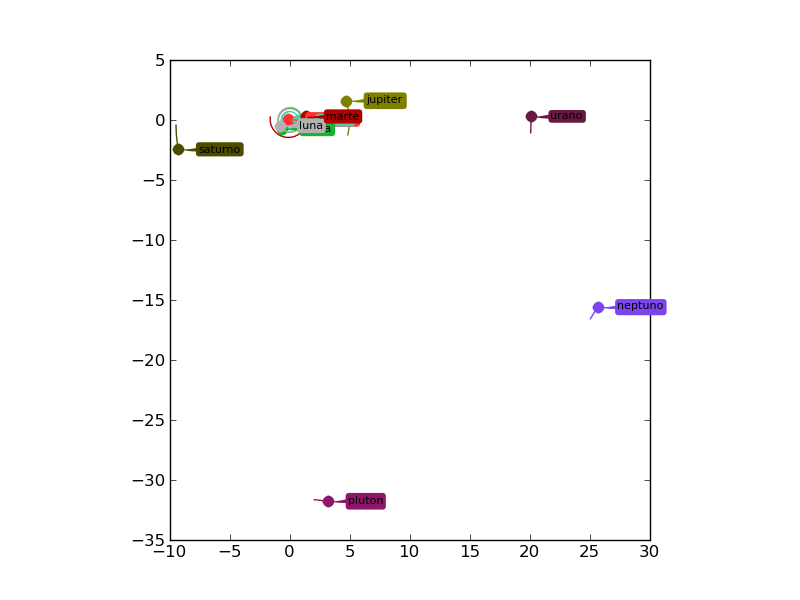
\includegraphics[scale=0.38]{img/ej2/metodo_2/validacion_365_12.png}
	\label{fig:ej2_m2_365_12}
	}
	\subfigure[$\Delta t$ = 1 hora]{
	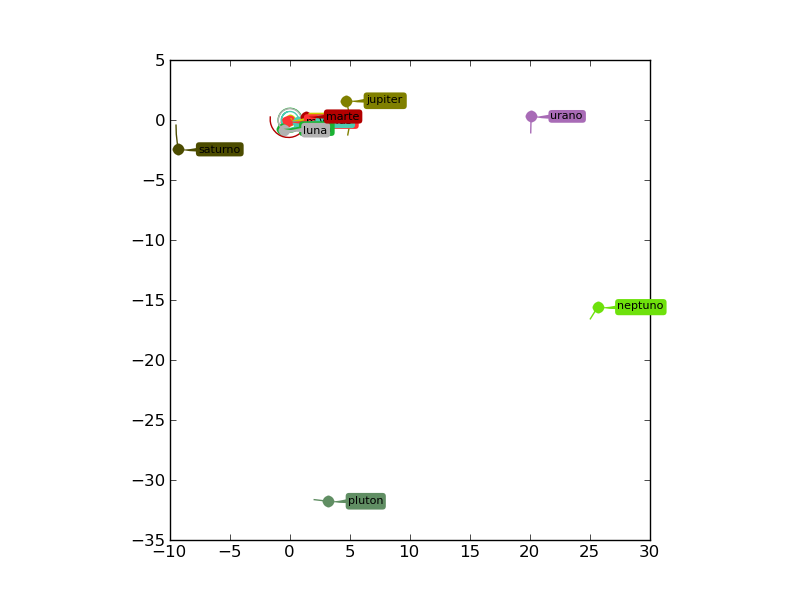
\includegraphics[scale=0.38]{img/ej2/metodo_2/validacion_365_24.png}
	\label{fig:ej2_m2_365_24}
	}
	\caption{
		Simulación de validación del sistema solar para un período de 1 año y distintos $\Delta t$
		con el método 2.
		Otra vez no hay mucho que ver para este período de tiempo.
	}
	\label{ fig:res_ej2_m2_365 }
\end{figure}
\begin{figure}
	\centering
	\subfigure[$\Delta t$ = 1 día]{
	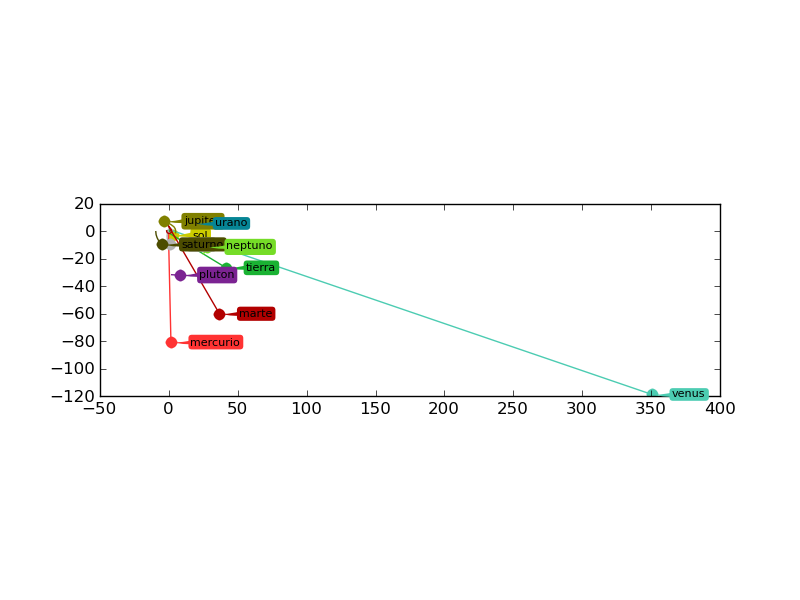
\includegraphics[scale=0.38]{img/ej2/metodo_2/validacion_1825_1.png}
	\label{fig:ej2_m2_1825_1}
	}
	\subfigure[$\Delta t$ = 6 horas]{
	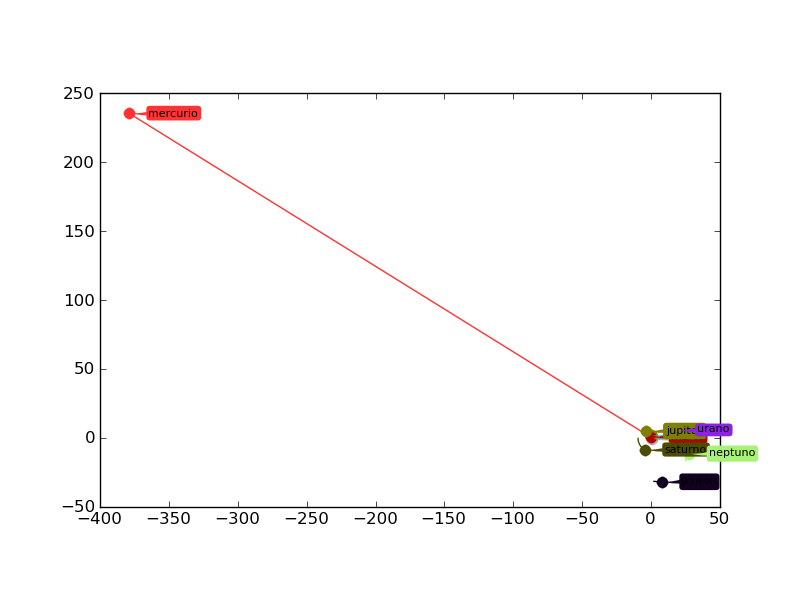
\includegraphics[scale=0.38]{img/ej2/metodo_2/validacion_1825_4.png}
	\label{fig:ej2_m2_1825_4}
	}
	\\
	\subfigure[$\Delta t$ = 2 horas]{
	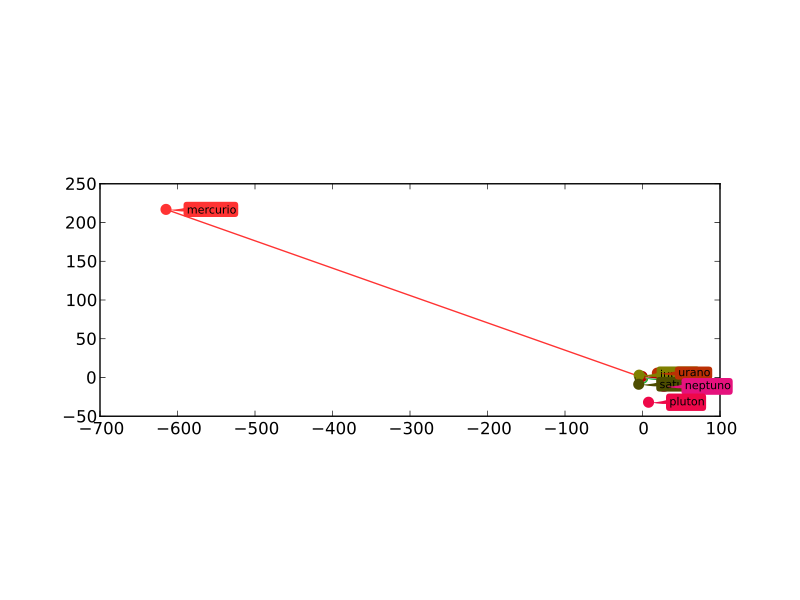
\includegraphics[scale=0.35]{img/ej2/metodo_2/validacion_1825_12.png}
	\label{fig:ej2_m2_1825_12}
	}
	\subfigure[$\Delta t$ = 1 hora]{
	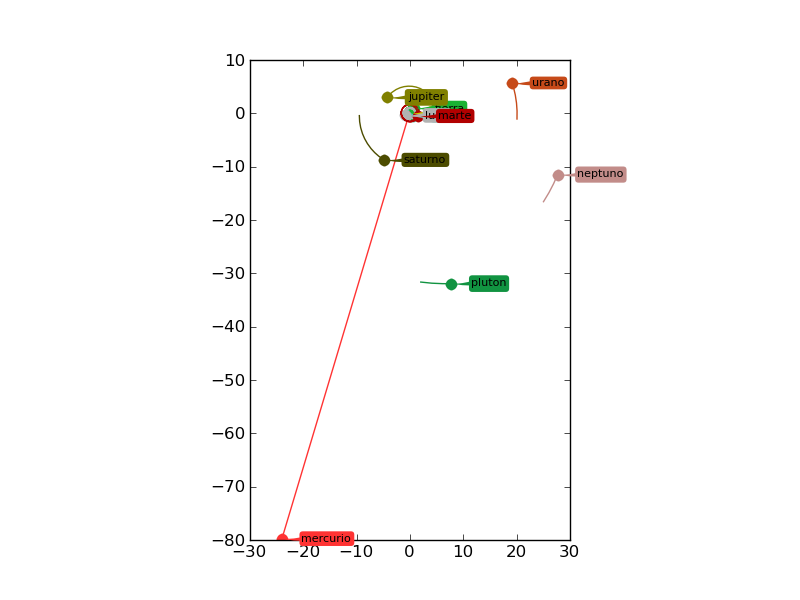
\includegraphics[scale=0.35]{img/ej2/metodo_2/validacion_1825_24.png}
	\label{fig:ej2_m2_1825_24}
	}
	\caption{
		Simulación de validación del sistema solar para un período de 5 años y distintos $\Delta t$
		con el método 2.
		Aquí vemos de nuevo lo sensible que es el segundo método a los errores producidos por la discretización del tiempo.
		Vemos como para mercurio se pierde totalmente la órbita
		(probablemente la causa es la proximidad de un cuerpo con mucha masa como el sol)
		y este sale disparado fuera del sistema. Al simular con mas definición, sin embargo, el producto mejora notablemente.
	}
	\label{ fig:res_ej2_m2_1825 }
\end{figure}
